%%This is a very basic article template.
%%There is just one section and two subsections.
\documentclass{article}
\usepackage[latin1]{inputenc} %coding of writteninput %latin1 allows for Umlaute
\usepackage[T1]{fontenc}%vectorized fonts (cm-super package)
\usepackage[german]{babel}%some specifics of the german language
\usepackage{amsfonts, amsmath, amsthm, amssymb, mathabx, paralist}
 \setlength{\parindent}{0em} 
  \usepackage{listings}
\usepackage{geometry}
  \geometry{a4paper, top=25mm, left=20mm, right=15mm, bottom=20mm, headsep=10mm, footskip=12mm}
 \usepackage{rotating} 
 %Decisiontree
 \usepackage{tikz,forest}
\usetikzlibrary{arrows.meta,arrows,shadows,positioning,decorations.pathreplacing}
\pgfdeclarelayer{background}
\pgfdeclarelayer{foreground}
\pgfsetlayers{background,main,foreground}
\usepackage{float}
\usepackage{enumitem}



  
\usepackage{graphicx} 

\usepackage{verbatim}%f�r txt datei

\usepackage{color} %red, green, blue, yellow, cyan, magenta, black, white
\definecolor{mygreen}{RGB}{28,172,0} % color values Red, Green, Blue
\definecolor{mylilas}{RGB}{170,55,241}

\usepackage[section]{placeins}

\begin{document}

\subsection*{Rapidminer}
For simplicity a powerful software system with a variety of different ways for clustering analysis, called Rapidminer Studio, is used to find correlations between spatio temporal data points. It enables to graphically form a pipeline from our spatio temporal input data to a concrete clustering by composing small blocks called \textbf{operators}. The first approach is to simply retrieve the base data from Medell�n and feed it into a clustering operator which uses K-means. 

\subsubsection*{Corrupted Data}
The first visible thing is that the data is corrupted, i. e. there are missing values for some data points, which are not allowed for the clustering operators. To fix this issue the missing values are replaced with the average value of the respective attribute. Furthermore it is not known if there are correlations between different data points, i. e. if two different data points are associated with the very same person, which is critical for clustering analysis to ensure that one person is not part of different clusters. Consider two travels, one at morning and one at midnight, which form a cycle, i. e. the start (end) of the first travel is equal to the end (start) of the second one. This type of correlation reflects, that people normally leave the house in the morning and get home at the end of the day, which is not well handled by the Euclidian Distance and could lead to bad clustering.

%Since the data has both categorical and numerical values, the mixed euclidian distance is used as similarity measure to calculate the difference between two data points with both numerical and categorical attributes.
%
%\subsubsection*{Mixed Euclidian Distance}
%The Euclidian distance for numerical vectors is given by
%$$d(p,q) = \sqrt{(p_1-q_1)^2+...+(p_n-q_n)^2} \text{ with }p=(p_1,...,p_n) \text{and }q=(q_1,...,q_n)$$
%which can be extended to measure the similarity of mixed vectors with both numerical and categorical types by defining
%$$(p_i-q_i)^2 = \begin{cases}
%0,& \text{if } p_i=q_i\\
%1,& \text{otherwise}\\
%\end{cases}$$ as distance between two categorical values.

\subsection*{Data Analysis}
\begin{minipage}[c]{0.48\textwidth}
\begin{figure}[H]
	\centering

		\centering
		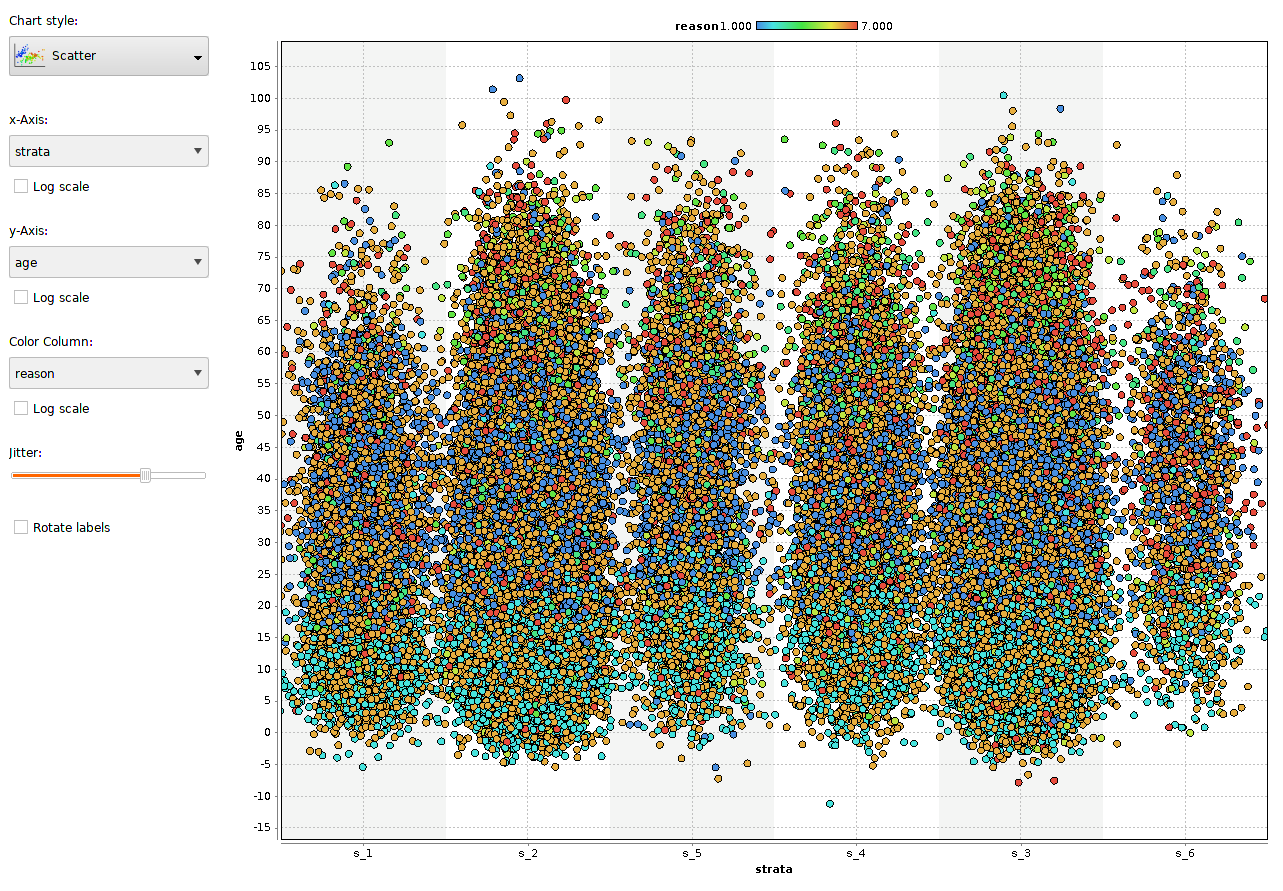
\includegraphics[width=3.0in]{../Martin-RapidMiner/diagramme/strata_age_reasonLearnWorkRetire.png}
		\caption{Reason for movement of people at different ages grouped by strata}
		\label{fig:strata_reason_age}

\end{figure}
\begin{figure}[H]
	\centering
	
	\centering
	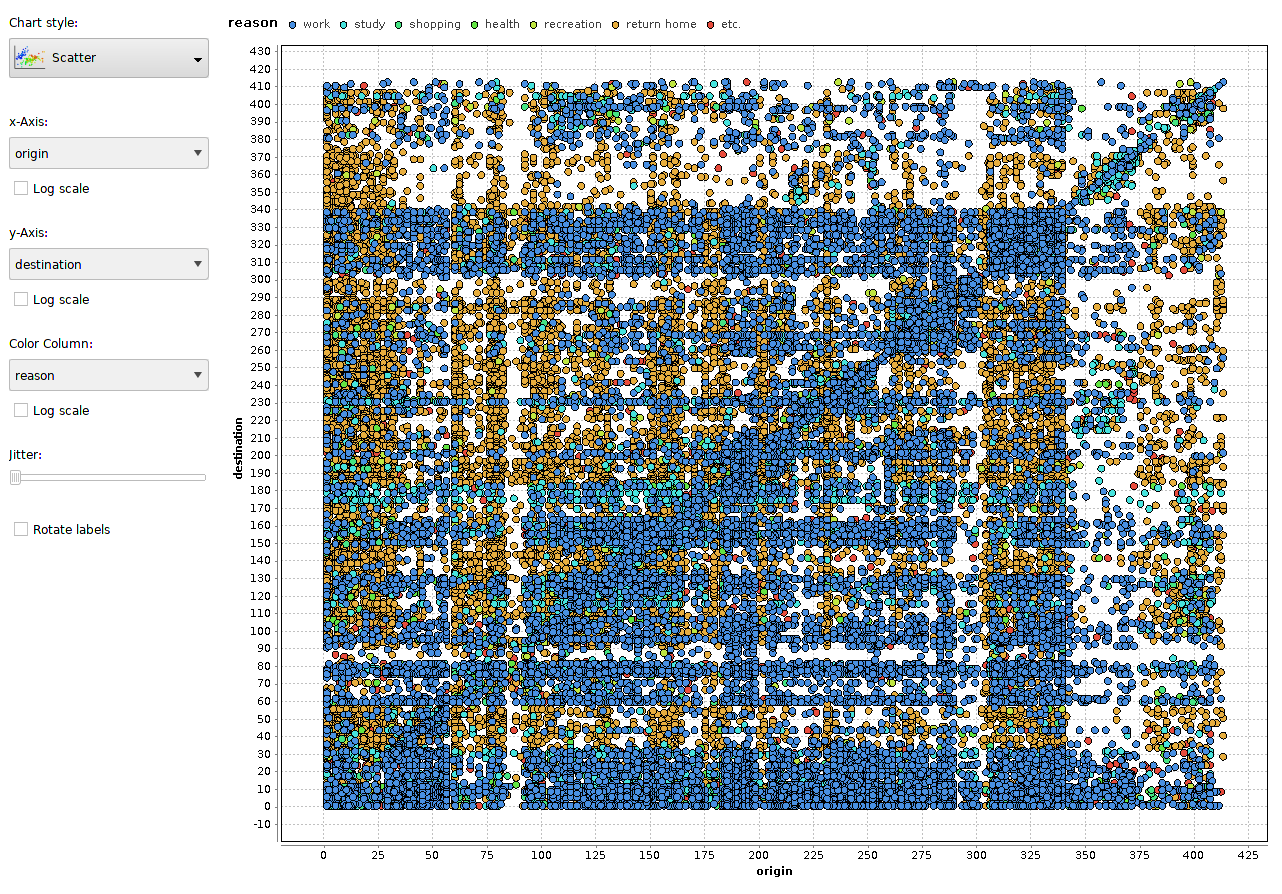
\includegraphics[width=3.0in]{../Martin-RapidMiner/diagramme/origin_destination_reason_lowJitter.png}
	\caption{Reason for movements from origin to destination}
	\label{fig:origin_destination_reason}
	
\end{figure}
	\end{minipage}
\begin{minipage}{0.48\textwidth}
	We are looking for clusters inside the whole dataset by generating different charts which visualize a subset of attributes of all data points. Firstly, before neglecting the strata data of the data set, we consider chart \ref{fig:strata_reason_age} which visualizes the different reasons why people move at which age grouped by socio-economic classes. Throughout the classes each cloud of points is very similar, i. e. young people are mostly studying, adults are mostly working and older people are moving for recreation or health. Therefore categorizing people by taking the reason for their movements into account is not an option. The only difference that is not caused by outliers is the smaller size of the first and last economic class.\\
	
	In figure \ref{fig:origin_destination_reason} we see the reason (color of dots) why people move from their origin to a destination. It can be seen, that the vast majority of people is working and that there are metropoliton areas inside the city. Some areas, for example around 180, tend to be more visited for academic purposes but since no matter what socio-economic strata people belong, they educate themselves i. e. there is not enough correlation between origin, destination and reason to see clusters which resemble the stratification just by plotting the data in this way. As in the original paper stated (TOOD: cite), there are differences between the stratas, which can be seen when plotting the strata as color column. For example plotting the means of transportation and the reason of travel by taking an equally distributed subset of the data set into account, the richest and poorest people have the most remarkable properties, i. e. the population of strata 1 is only working, studying and returning home by using first and second means of transportation, whilst the reasons for movements of people from strata 6 are more spread but mostly using the third means of transportation, which seems to be only affordable for wealthy people.	 
\end{minipage}\\

We observe, that there are visible differences between the different given stratifications. But since the population of each strata is not homogenous and the clear distinction of two succeeding is not given, we can not see clusters by plotting the data without knowing the result. In the following sections we are therefore investigating approaches to find clusters using different clustering algorithms.



%\begin{enumerate}
	
%	\item Exponential distribution of travels regarding traveling distance\\\\
	
%	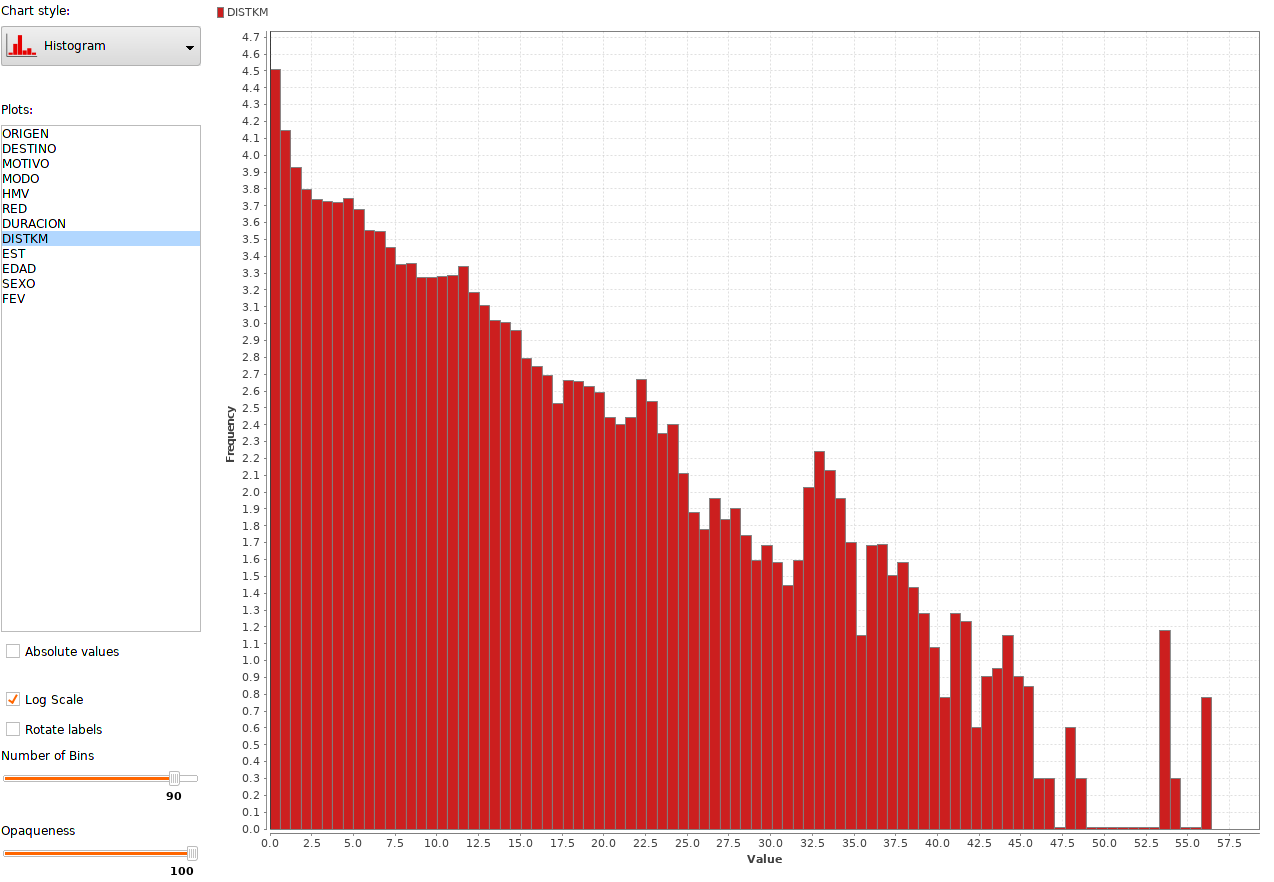
\includegraphics[width=0.5\textwidth]{data_findings/exponential distr.png}
%\end{enumerate}

\end{document}













